\chapter{Methods}\label{ch:methods}

\begin{chapterabstract}
    In the following chapter, we outline the methods of work used to assess the Gaia-X initiative, the reference framework implementation by GXFS and answer the research questions stated in the introductory Chapter~\ref{ch:introduction}.
    The main method of work is implementation of a Gaia-X-compliant data exchange module, serving as a proof of concept.
    Based on this, we note the Gaia-X related technical challenges.
    Additionally, we take a closer look on the architecture of Gaia-X and at the project in which we implement the data exchange module.
    Lastly, we present a selection of risks and metrics identified in the previous Chapter~\ref{ch:related-work} --- Related Work.
\end{chapterabstract}

\section{About Carecentive}\label{sec:about-carecentive}

Carecentive~\cite{carecentive} is a backend software framework used for supporting health studies and trials.
The framework offers features that are typically required in medical trials, notably the following:
\begin{itemize}
    \item User management (registration, login, password management)
    \item Questionnaire storage \& submission
    \item Activity scheduling (e.g., periodical questionnaire submission)
    \item File upload (e.g., images of medical records)
    \item Wearable devices integration (Withings API, Fitbit API)
    \item User activity analytics
    \item Permission management (Roles such as patients, relatives, physicians, nurses, study managers)
\end{itemize}

\subsection{Tech Stack}\label{subsec:tech-stack}

From the developmental standpoint, the framework is divided into two packages, \textit{carecentive-framework}\footnote{https://github.com/carecentive/carecentive-framework} which mainly sets up the application, registers and exposes the API on the outside.
The API requests are then handed over to the main package \textit{carecentive-code}\footnote{https://github.com/carecentive/carecentive-core}, which does the heavy lifting of handling user requests based on its business logic.

The Carecentive is written in the \textit{JavaScript} programming language and is running in the \textit{Node.js} engine.
It is built on top of the \textit{Express} web framework, enabling the RESTful API interface, stores data in the relational MySQL DBMS (Database Management Systems).
The database tables are versioned via database migrations enabled by the\textit{Knex.js} library, and relational data is mapped onto objects (models) using the \textit{Objection.js} library.

%TODO: add references to the libraries
In order to simplify setting up the project on different machines and improve stability, we also used the Docker platform, which ensures installation of all dependencies and runs the app in an isolated environment, reducing the differences in various operating systems.
%TODO: should I explain this more?

\subsection{Use Cases}\label{subsec:use-cases}

The framework was developed at FAU MaD Lab, under which I'm working on this thesis.
Currently, a smartphone app is used as a frontend for the Carecentive backend counterpart in a running study investigating the health of patients receiving care at the palliative care unit in the \textit{Uniklinikum Erlangen} (University Hospital Erlangen).
Thanks to the extensibility of the Carecentive framework, it was also utilized in the works of other students doing their thesis under the FAU MaD Lab (e.g., Smartphone-based Urinalysis).

%TODO: add screenshots of the app

In order to assess the functionality of the Gaia-X ecosystem, a partial goal of this thesis is to implement a Gaia-X-compliant module for the exchange of the data stored in the Carecentive app.
During the implementation of the exchange module, serving as a proof of concept, we note of any technical or other issues with the Gaia-X specifications and with the GXFS software.
After the implementation is finished, we run a set of predefined data exchange scenarios to verify the correct functionality of our implementation and mainly whether the Gaia-X and GXFS software is ready for a real-world usage.
This is done with in the specific use-case of the palliative care trial.

\section{Gaia-X Concepts}\label{sec:gaia-x-concepts}

\subsection{Credentials}\label{subsec:credentials}

%TODO: replace Self-Desctiptions with Gaia-X Credentials
Gaia-X Credentials, formerly known as Gaia-X Self-Descriptions, are the main conceptual building blocks of the Gaia-X ecosystem~\cite{gaiax_architecture_document}.
They formalize all the claims and descriptions made by all parties participating in the ecosystem.
They are based on the formal \textit{Verifiable Credentials Data Model}~\cite{verifiable_credentials} specification issued by the \textit{World Wide Web Consortium} (W3C) and on the concept of Linked Data (LD).

Verifiable Credentials are inspired by physical credentials like government-issued passports, driving licenses and university diplomas.
They contain information about some statements the credential holder is trying to prove (citizenship, achieved education, etc.) and are secured by some protective element from the issuer, proving the veracity of the document, which the verifier can verify.
Their software counterpart (VCs) work in a similar way.
They contain data with relevance to the holder, which is structured based on well-defined templates called schemas or vocabularies, which describe which claims can be made in the document.

The claim consists of a subject (credential holder), property and a value, for example, Pat being an alumni of ``Example University''~\ref{fig:verifiable-credential-claim}.
These claims are then packed into the credential body along with metadata such as the issuer, issuance date or the expiration date.
Although other formats are permitted, the base format VCs are encoded in is the JSON (JavaScript Object Notation) format or more specifically the extension for Linked Data --- JSON-LD, this ensures the data is machine-readable and can be interlinked between each other.
The issuer then signs the credential using digital signature proving, which is inserted into the VC's proof section.
This provides a machine-readable cryptographical proof, which secures the credential and can be used by the verifier to verify holder's claims.

\begin{figure}
    \centering
    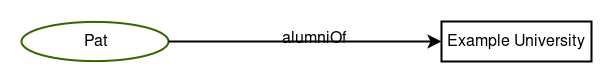
\includegraphics[width=\textwidth]{figures/verifiable-credential-claim-example.png}
    \caption{An example claim expressing Pat being an alumni of ``Example University''~\cite{verifiable_credentials}}\label{fig:verifiable-credential-claim}
\end{figure}
%TODO: fix svg figures
\begin{figure}
    \centering
    
\includegraphics[width=\textwidth]{figures/verifiable-credentials.png}
    \caption{Verifiable Credential roles and information flow~\cite{verifiable_credentials}}\label{fig:verifiable-credentials}
\end{figure}

Gaia-X utilizes VCs for almost all of the objects in the ecosystem from the \texttt{Participant}, serving as a description of a natural person or a legal entity, to the \texttt{ServiceOffering} and \texttt{Resource} credentials, specifying the offered services or data.
Gaia-X provides the so-called \textit{Gaia-X Trust Framework} via which the syntactic correctness, schema validity, cryptographic signature validation, attribute value consistency and attribute value verification is enforced~\cite{gaiax_architecture_document}.
This is done to ensure compliance with the minimal requirements defined by Gaia-X specifications is met.
However, thanks to the possible extensibility of the VC schemas, each federation can impose new rules for the credentials which federation Participants have to obey.

\begin{figure}
\centering
\begin{minted}[bgcolor=LightGray,breaklines]{json}
{
  "@context": [
    "https://www.w3.org/2018/credentials/v1",
    "https://w3id.org/security/suites/jws-2020/v1",
    "https://registry.lab.gaia-x.eu/development/api/trusted-shape-registry/v1/shapes/jsonld/trustframework#"
  ],
  "type": [
    "VerifiableCredential"
  ],
  "id": "https://gaia-x-dev.simerda.dev/gaia-x/john-doe/participant.json",
  "issuer": "did:web:gaia-x-dev.simerda.dev:gaia-x:john-doe",
  "issuanceDate": "2024-08-13T17:50:27.483+00:00",
  "credentialSubject": {
    "id": "https://gaia-x-dev.simerda.dev/gaia-x/john-doe/participant.json#cs",
    "type": "gx:LegalParticipant",
    "gx:legalName": "Example Enterprise",
    "gx:legalRegistrationNumber": {
      "id": "https://gaia-x-dev.simerda.dev/gaia-x/john-doe/legal-registration-number.json#cs"
    },
    "gx:headquarterAddress": {
      "gx:countrySubdivisionCode": "CZ-52"
    },
    "gx:legalAddress": {
      "gx:countrySubdivisionCode": "CZ-52"
    }
  },
  "proof": {
    "created": "2024-08-13T17:50:28.392+00:00",
    "type": "JsonWebSignature2020",
    "proofPurpose": "assertionMethod",
    "verificationMethod": "did:web:gaia-x-dev.simerda.dev:gaia-x:john-doe#JWK2020-RSA",
    "jws": "eyJhbGciOiJQUzI1NiIsImI2NCI6ZmFsc2UsImNyaXQiOlsiYjY0Il19..cPShjGoSpCKGfjU6pvjQnGeXCiN36smCdSpkPwp6Ruf24bSzvKQ2Slg9mve84-ZbEaVJVhtn6q1p833xaCAI9m0h3EUnzctukottOGrdWD5pJG2EHwkDYYY_SrfOT_Y7uIYaSf46_2FPAzvHxGoTRGPkvR-6cPmV_RW6Js6iagqmeOY1zjV89q4_2HibNnGWRLIAlWs1yrwk-3w4JEQWgQcilCa3xy_9i7L3mWyVE_4JC0HvXGVvanViIbr04xHdf--AkPlgO-eBItDogjL7pcUf0R7ORgB_ho7lP6OfbKht8Ru5PXNQjgfFJ2TO7zw9sJmaCRCqenCjn-QpfniMuA"
  }
}
\end{minted}
\caption{Example of a Gaia-X Participant Credential}\label{fig:gaia_x_credential_example}
\end{figure}

Following general types of Gaia-X Credentials are defined~\cite{gaiax_architecture_document,gaiax_trust_framework}:
\begin{itemize}
    \item \textbf{Participant} --- Represents a participant onboarded into the Gaia-X ecosystem.
    Participants can either be a LegalPerson or a NaturalPerson and are always interlinked to the ServiceOfferings they are providing.
    \item \textbf{LegalRegistrationNumber} --- Represents a registration number of a legal entity and must be linked to the LegalPerson type of the Participant credential.
    It can be one of the following numbers:
    \begin{itemize}
        \item \textbf{local}: a state issued company number
        \item \textbf{EUID}: a unique identifier for businesses located in the EEA
        \item \textbf{EORI}: the Economic Operators Registration and Identification number
        \item \textbf{vatID}: the VAT identification number
        \item \textbf{leiCode}: the LEI (Legal Entity Identifier) code as defined by \url{https://www.gleif.org}
    \end{itemize}
    \item \textbf{GaiaXTermsAndConditions} --- Represents a Participant's agreement to the Gaia-X terms and conditions and commits to keep its Gaia-X Credentials up-to-date.
    The \textit{Gaia-X Association} may revoke the keypair used to sign the VC upon failure to comply with these rules.
    \item \textbf{Resource} --- Represents a resource a Participant desires to make available.
    It can be of the type PhysicalResource, which is related to a hardware component occupying physical space (e.g., a data center, a hardware service, a plant,~\ldots), or of the VirtualResource type, which describes virtual artifacts (e.g., a dataset, software, a configuration file, and AI model,~\ldots).
    \item \textbf{ServiceOffering} --- Represents an aggregation of Resource Credentials and defines terms and conditions of usage.
    ServiceOffering is the main credential used to promote an offered service.
    It can be exposed on the provider's web server or published in a federated catalogue to allow searchability and findability.
    \item \textbf{ServiceInstance} --- Represents a running instance of a Virtual Resource; hence, it's also known as an \textit{Instantiated Virtual Resource}.
    It is mainly used for instantiating a \textit{Software Resource}.
\end{itemize}

The relations between credentials can be seen visually in a diagram in Figure~\ref{fig:credential_relations}.

\begin{figure}
    \centering
    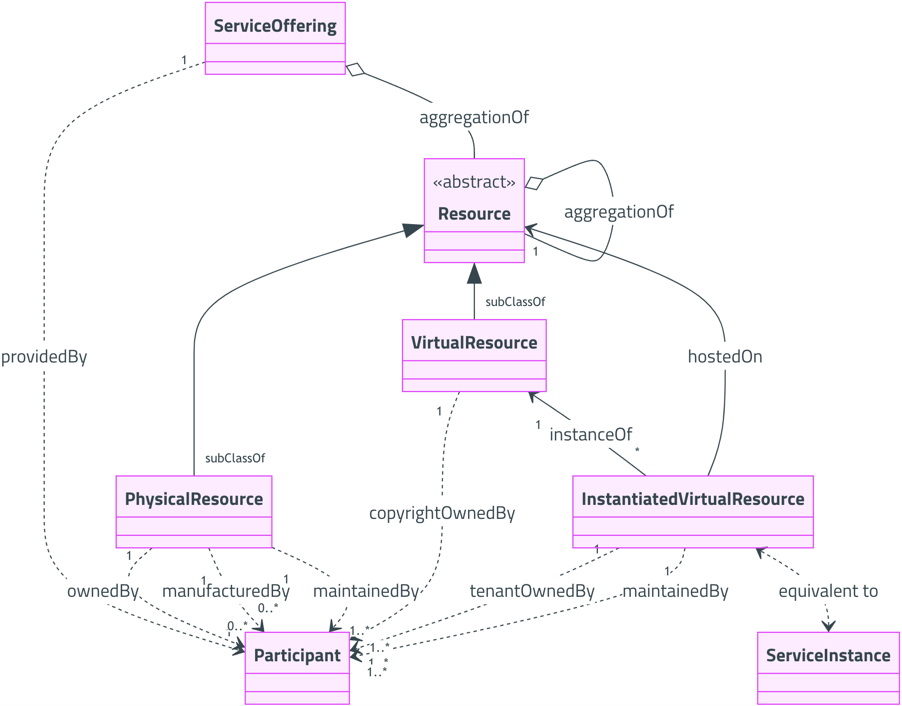
\includegraphics[width=\textwidth]{figures/credential-relations.png}
    \caption{Relations between different types of Gaia-X Credentials~\cite{gaiax_architecture_document}}\label{fig:credential_relations}
\end{figure}

Let's now examine each of the Credentials individually and their attributes.
The LegalRegistrationNumber Credential is omitted since it's issued by the Gaia-X Notary service based on the provided registration number and its successful validation and not self-signed by the participant.
Further information about the Notary service is provided in section~\ref{subsec:trust-framework-components}.

\subsubsection{Participant}

\begin{longtable}{ |p{4cm}|p{2cm}|p{2cm}|p{7cm}| }
    \hhline{----}
    \textbf{Attribute} & \textbf{Mandatory} & \textbf{Multiple values allowed} & \textbf{Description}\\
    \hhline{----}
    \texttt{registrationNumber} & Yes & No & Unique registration number of the legal entity\\
    \hhline{----}
    \texttt{headquartersAddress.countryCode} & Yes & No & Country code of the company's headquarters in ISO 3166--2 format\\
    \hhline{----}
    \texttt{legalAddress.countryCode} & Yes & No & Country code of the company's legally registered address in ISO 3166--2 format\\
    \hhline{----}
    \texttt{parentOrganization} & No & Yes & List of direct Participants this entity is a subOrganization of\\
    \hhline{----}
    \texttt{parentOrganization} & No & Yes & List of direct Participants with a legal mandate on this entity (e.g., subsidiaries)\\
    \hhline{----}
    \caption{Participant Gaia-X Credential attributes~\cite{gaiax_trust_framework}}
    \label{tab:participant}
\end{longtable}

\subsubsection{Resource}

\begin{longtable}{ |p{4cm}|p{2cm}|p{2cm}|p{7cm}| }
    \hhline{----}
    \textbf{Attribute} & \textbf{Mandatory} & \textbf{Multiple values allowed} & \textbf{Description}\\
    \hhline{----}
    \texttt{aggregationOf} & No & Yes & Resources related to the Resource and that can exist independently of it\\
    \hhline{----}
    \texttt{name} & No & No & A human readable name of the Resource\\
    \hhline{----}
    \texttt{description} & No & No & A free-text description of the Resource\\
    \hhline{----}
    \caption{Resource Gaia-X Credential attributes~\cite{gaiax_trust_framework}}
    \label{tab:resource}
\end{longtable}

\subsubsection{Physical Resource}

Physical Resource inherits from the Resource Credential and defines the following extra attributes~\cite{gaiax_trust_framework}.

\begin{longtable}{ |p{4cm}|p{2cm}|p{2cm}|p{7cm}| }
    \hhline{----}
    \textbf{Attribute} & \textbf{Mandatory} & \textbf{Multiple values allowed} & \textbf{Description}\\
    \hhline{----}
    \texttt{maintainedBy} & Yes & Yes & A list of Participants maintaining the Resource operational and having physical access to it\\
    \hhline{----}
    \texttt{ownedBy} & No & Yes & A list of Participants owning the Resource\\
    \hhline{----}
    \texttt{manufacturedBy} & No & Yes & A list of Participants manufacturing the Resource\\
    \hhline{----}
    \texttt{locationAddress[].countryCode} & Yes & Yes & A list of physical locations' country codes of the Resource in ISO 3166--2 format\\
    \hhline{----}
    \texttt{location[].gps} & No & Yes & A list of physical locations' GPS coordinates of the Resource in ISO 6709:2008/Cor~1:2009 format\\
    \hhline{----}
    \caption{PhysiscalResource Gaia-X Credential attributes~\cite{gaiax_trust_framework}}
    \label{tab:physical_resource}
\end{longtable}

\subsubsection{Virtual Resource}

Virtual Resource inherits from the Resource Credential and defines the following extra attributes~\cite{gaiax_trust_framework}.

\begin{longtable}{ |p{4cm}|p{2cm}|p{2cm}|p{7cm}| }
    \hhline{----}
    \textbf{Attribute} & \textbf{Mandatory} & \textbf{Multiple values allowed} & \textbf{Description}\\
    \hhline{----}
    \texttt{copyrightOwnedBy} & Yes & Yes & A list of copyright owners of the Resource either as a free-text or as URLs from which can be resolved to the Participant Credential\\
    \hhline{----}
    \texttt{license} & Yes & Yes & A list of licenses either as SPDX\footnote{\url{https://spdx.org/licenses/}} identifiers or a URL to the license document\\
    \hhline{----}
    \texttt{policy} & Yes & Yes & A list of policies specified as described in section~\ref{subsec:policies}\\
    \hhline{----}
    \caption{VirtualResource Gaia-X Credential attributes~\cite{gaiax_trust_framework}}
    \label{tab:virtual_resource}
\end{longtable}

\subsubsection{Data Resource}

Data Resource inherits from the Virtual Resource Credential and defines the following extra attributes~\cite{gaiax_trust_framework}.

\begin{longtable}{ |p{4cm}|p{2cm}|p{2cm}|p{7cm}| }
    \hhline{----}
    \textbf{Attribute} & \textbf{Mandatory} & \textbf{Multiple values allowed} & \textbf{Description}\\
    \hhline{----}
    \texttt{producedBy} & Yes & No & A resolvable link to the Participant's Credential legally enabling the data usage\\
    \hhline{----}
    \texttt{exposedThrough} & Yes & Yes & A list resolvable links to the data exchange component that exposes the data resource\\
    \hhline{----}
    \texttt{obsoleteDateTime} & No & No & Date and time in ISO 8601 format after which data is obsolete\\
    \hhline{----}
    \texttt{expirationDateTime} & No & No & Date and time in ISO 8601 format after which data is expired and shall be deleted\\
    \hhline{----}
    \texttt{containsPII} & Yes & No & Whether the Resource contains \textit{Personally Identifiable Information}\\
    \hhline{----}
    \texttt{legalBasis} & Yes if containsPII & No & Reason for data collection in the Data Protection Regimes such as GDPR. Potential legal bases can be article 6, article 7 or article 9.
    It shall be expressed as a string matching \texttt{6.1.[a-f]}, \texttt{6.1.4}, \texttt{7} or \texttt{9.2.[a-j]}\\
    \texttt{dataProtectionContact} & Yes if containsPII & No & Means to raise personal data-protection-questions related to the data source.
    Either a URL resolved to a contact form or an email address\\
    \hhline{----}
    \caption{DataResource Gaia-X Credential attributes~\cite{gaiax_trust_framework}}
    \label{tab:data_resource}
\end{longtable}

\subsubsection{Software Resource}

Software Resource inherits from the Virtual Resource Credential and doesn't define any extra attributes.

\subsubsection{Service Offering}

\begin{longtable}{ |p{4cm}|p{2cm}|p{2cm}|p{7cm}| }
    \hhline{----}
    \textbf{Attribute} & \textbf{Mandatory} & \textbf{Multiple values allowed} & \textbf{Description}\\
    \hhline{----}
    \texttt{name} & No & No & A human readable name of the ServiceOffering\\
    \hhline{----}
    \texttt{providedBy} & Yes & No & A resolvable link to the Participant's Credential providing the service\\
    \hhline{----}
    \texttt{aggregationOf} & No & Yes & A resolvable link to the Resource Credentials related to the service\\
    \hhline{----}
    \texttt{dependsOn} & No & Yes & A resolvable link to the ServiceOffering Credentials related to the service and that can exist independently of it\\
    \hhline{----}
    \texttt{termsAndConditions} & Yes & Yes & A resolvable link to the terms and conditions applying to the service.
    Consists of \texttt{URL} and \texttt{hash}\\
    \hhline{----}
    \texttt{policy} & Yes & Yes & A list of policies specified as described in section~\ref{subsec:policies}\\
    \hhline{----}
    \texttt{dataProtectionRegime} & No & Yes & A data protection regime used for the data (e.g., \textit{GDPR2016}, \textit{LGPD2019}, \textit{PDPA2012}, \textit{CCPA2018}, \textit{VCDPA2021})\\
    \hhline{----}
    \texttt{dataAccountExport[].requestType} & Yes & Yes & Request type for exporting personal and non-personal data out of the service.
    One of \texttt{API}, \texttt{email}, \texttt{webform}, \texttt{unregisteredLetter}, \texttt{registeredLetter}, \texttt{supportCenter}\\
    \hhline{----}
    \texttt{dataAccountExport[].accessType} & Yes & Yes & Type of data support for exporting personal and non-personal data out of the service.
    One of (\texttt{digital}, \texttt{physical})\\
    \hhline{----}
    \texttt{dataAccountExport[].formatType} & Yes & Yes & Type of format for the export of personal and non-personal data out of the service.
    Must be one of the Media Types\footnote{\url{https://www.iana.org/assignments/media-types/media-types.xhtml}} as defined by IANA\\
    \hhline{----}
    \caption{ServiceOffering Gaia-X Credential attributes~\cite{gaiax_trust_framework}}
    \label{tab:service_offering}
\end{longtable}

\subsubsection{Service Instance}

\begin{longtable}{ |p{4cm}|p{2cm}|p{2cm}|p{7cm}| }
    \hhline{----}
    \textbf{Attribute} & \textbf{Mandatory} & \textbf{Multiple values allowed} & \textbf{Description}\\
    \hhline{----}
    \texttt{maintainedBy} & Yes & Yes & A list of Participants maintaining the Instantiated Virtual Resource operational\\
    \hhline{----}
    \texttt{hostedOn} & Yes & No & A Physical Resource, where the process is located\\
    \hhline{----}
    \texttt{instanceOf} & Yes & No & A resolvable link to the Virtual Resource Credential (normally a Software Resource) this process is an instance of\\
    \hhline{----}
    \texttt{dependsOn} & No & Yes & A resolvable link to the ServiceOffering Credentials related to the service and that can exist independently of it\\
    \hhline{----}
    \texttt{tenantOwnedBy} & Yes & Yes & A list of Participants with contractual relation to the Resource\\
    \hhline{----}
    \texttt{serviceAccessPoint} & Yes & Yes & A list of objects specifying a service access point (endpoint or other means of interaction with the resource)\\
    \hhline{----}
    \caption{ServiceInstance Gaia-X Credential attributes~\cite{gaiax_trust_framework}}
    \label{tab:service_instance}
\end{longtable}

\subsubsection{Data Exchange Credentials}

In the context of data offerings and data exchange, another set of Gaia-X Credentials is defined in the \textit{Data Exchange Services Specifications} document~\cite{gaiax_data_exchange_document}.
The document introduces new Participant roles (\texttt{DataProductProvider}, \texttt{DataLicensor}, \texttt{DataProducer} and \texttt{DataConsumer}) and specifies Credentials describing data, the dataset, its distribution and the possible contract between Data Consumer and Data Product Provider.
Following data-exchange-specific types of Gaia-X Credentials are defined~\cite{gaiax_data_exchange_document}:
\begin{itemize}
    \item \textbf{DataProductDescription} --- Inherits the attributes of the ServiceOffering Credential and also extends the W3C Data Catalog Vocabulary (DCAT) Resource class\footnote{\url{https://www.w3.org/TR/vocab-dcat-3/\#Class\%3AResource}}.
    \item \textbf{DatasetDescription} --- Represents a description of the offered dataset.
    Extends attributes of the W3C DCAT Dataset class\footnote{\url{https://www.w3.org/TR/vocab-dcat-3/\#Class\%3ADataset}}.
    \item \textbf{DataUsage} --- Represents details related to data usage.
    Currently only an optional logging service can be specified.
    \item \textbf{DataProductUsageContract} --- Specifies the final contract between DataConsumer and DataProductProvider, allowing the consumer to use the data.
\end{itemize}

Let's now examine each of the data-exchange-related Credentials individually along with their attributes.

\subsubsection{DataProductDescription}

Data Product Description inherits Service Offering Credentials and defines the following attributes~\cite{gaiax_data_exchange_document}.

\begin{longtable}{ |p{4cm}|p{2cm}|p{2cm}|p{7cm}| }
    \hhline{----}
    \textbf{Attribute} & \textbf{Mandatory} & \textbf{Multiple values allowed} & \textbf{Description}\\
    \hhline{----}
    \texttt{providedBy} & Yes & No & A resolvable link to the Participant's Credential providing the data\\
    \hhline{----}
    \texttt{termsAndConditions} & Yes & No & A resolvable link to the terms and conditions applying to the service\\
    \hhline{----}
    \texttt{license} & Yes & Yes & A list of URLs to the license documents\\
    \hhline{----}
    \texttt{title} & Yes & No & A human readable title of the Data Product\\
    \hhline{----}
    \texttt{description} & No & No & A free-text description of the Data Product\\
    \hhline{----}
    \texttt{issued} & No & No & Date and time in ISO 8601 format of when the data was issued\\
    \hhline{----}
    \texttt{obsoleteDateTime} & No & No & Date and time in ISO 8601 format of when the data is obsolete\\
    \hhline{----}
    \texttt{hasPolicy} & No & No & A policy specified as described in section~\ref{subsec:policies}\\
    \hhline{----}
    \texttt{dataLicensors} & No & Yes & A list of resolvable links to the data licensors Participants' Credentials or a free-form string\\
    \hhline{----}
    \texttt{dataUsageAgreement} & Yes if containsPII & Yes & A list of authorizations from the data subjects as Natural Person
    Specified as the \texttt{DataUsageAgreement} object\\
    \hhline{----}
    \texttt{aggregationOf} & Yes & Yes & A list of resolvable links to the DatasetDescription Credentials\\
    \hhline{----}
    \texttt{identifier} & Yes & No & A unique UUID4 identifier\\
    \hhline{----}
    \texttt{contactPoint} & No & No & A contact to get more information in vCard format\\
    \hhline{----}
    \texttt{conformsTo} & No & Yes & List of established standards the data conforms to\\
    \hhline{----}
    \caption{DataProductDesctiption Gaia-X Credential attributes~\cite{gaiax_data_exchange_document}}
    \label{tab:data_product_description}
\end{longtable}

\subsubsection{DatasetDescription}

Data Product Description inherits Service Offering Credentials and defines the following attributes~\cite{gaiax_data_exchange_document}.

\begin{longtable}{ |p{4cm}|p{2cm}|p{2cm}|p{7cm}| }
    \hhline{----}
    \textbf{Attribute} & \textbf{Mandatory} & \textbf{Multiple values allowed} & \textbf{Description}\\
    \hhline{----}
    \texttt{title} & Yes & No & A human readable title of the Dataset\\
    \hhline{----}
    \texttt{distributions} & Yes & Yes & A list of descriptions of the dataset distributions\\
    \hhline{----}
    \texttt{identifier} & Yes & No & A unique UUID4 identifier\\
    \hhline{----}
    \texttt{issued} & No & No & Date and time in ISO 8601 format of when the data was issued\\
    \hhline{----}
    \texttt{expirationDateTime} & No & No & Date and time in ISO 8601 format of when the data is expired and shall be deleted\\
    \hhline{----}
    \texttt{license} & No & Yes & A list of URLs to the license documents\\
    \hhline{----}
    \texttt{dataLicensors} & No & Yes & A list of resolvable links to the data licensors Participants' Credentials or a free-form string\\
    \hhline{----}
    \texttt{dataUsageAgreement} & Yes if containsPII & Yes & A list of authorizations from the data subjects as Natural Person
    Specified as the \texttt{DataUsageAgreement} object\\
    \hhline{----}
    \texttt{exposedThrough} & Yes & Yes & A list of resolvable links to the data exchange component that exposes the dataset\\
    \hhline{----}
    \caption{DatasetDescription Gaia-X Credential attributes~\cite{gaiax_data_exchange_document}}
    \label{tab:dataset_description}
\end{longtable}

\subsubsection{DataUsage}

\begin{longtable}{ |p{4cm}|p{2cm}|p{2cm}|p{7cm}| }
    \hhline{----}
    \textbf{Attribute} & \textbf{Mandatory} & \textbf{Multiple values allowed} & \textbf{Description}\\
    \hhline{----}
    \texttt{loggingService} & No & No & A link to the logging service\\
    \hhline{----}
    \caption{DataUsage Gaia-X Credential attributes~\cite{gaiax_data_exchange_document}}
    \label{tab:data_usage}
\end{longtable}

\subsubsection{DataProductUsageContract}

\begin{longtable}{ |p{4cm}|p{2cm}|p{2cm}|p{7cm}| }
    \hhline{----}
    \textbf{Attribute} & \textbf{Mandatory} & \textbf{Multiple values allowed} & \textbf{Description}\\
    \hhline{----}
    \texttt{providedBy} & Yes & No & A resolvable link to the Participant's Credential providing the data\\
    \hhline{----}
    \texttt{consumedBy} & Yes & No & A resolvable link to the Participant's Credential consuming the data\\
    \hhline{----}
    \texttt{dataProduct} & Yes & No & A resolvable link to the Data Product Description Credential subject to the contract\\
    \hhline{----}
    \texttt{signers} & Yes & Yes & A list of Signature Check Type objects identifying all required Participant signatures\\
    \hhline{----}
    \texttt{termOfUsage} & Yes & No & A resolvable link to the term of usage\\
    \hhline{----}
    \texttt{notarizedIn} & No & No & A resolvable link to the Notarization service\\
    \hhline{----}
    \texttt{dataUsage} & Yes & No & A resolvable link to the Data Usage Credential\\
    \hhline{----}
    \caption{DataProductUsageContract Gaia-X Credential attributes~\cite{gaiax_data_exchange_document}}
    \label{tab:data_product_usage_contract}
\end{longtable}

\subsubsection{DistributionDescription}

Specifies mainly the dataset details related to the physical dataset file, like the format, hash and language,~\ldots.
It is not a standalone Gaia-X Credential, but an object needed to be specified in DatasetDescription Credential.

\begin{longtable}{ |p{4cm}|p{2cm}|p{2cm}|p{7cm}| }
    \hhline{----}
    \textbf{Attribute} & \textbf{Mandatory} & \textbf{Multiple values allowed} & \textbf{Description}\\
    \hhline{----}
    \texttt{title} & Yes & No & A human readable title of the Dataset\\
    \hhline{----}
    \texttt{format} & Yes & No & Dataset specified via the Media Types\footnote{\url{https://www.iana.org/assignments/media-types/media-types.xhtml}} as defined by IANA\\
    \hhline{----}
    \texttt{compressFormat} & No & No & The compression format used, in case the data is contained in compressed form\\
    \hhline{----}
    \texttt{packageFormat} & No & No & The package format of the distribution in which one or more data files are grouped together\\
    \hhline{----}
    \texttt{byteSize} & No & No & Size of the dataset distribution in bytes\\
    \hhline{----}
    \texttt{location} & No & Yes & A list of the dataset storage location\\
    \hhline{----}
    \texttt{hash} & No & No & A hash of the distribution to uniquely identify the data contained in the distribution\\
    \hhline{----}
    \texttt{hashAlgorithm} & No & No & An algorithm used to produce the hash value\\
    \hhline{----}
    \texttt{issued} & No & No & Date and time in ISO 8601 format of when the data was published\\
    \hhline{----}
    \texttt{expirationDateTime} & No & No & Date and time in ISO 8601 format of when the data is expired and shall be deleted\\
    \hhline{----}
    \texttt{language} & No & No & Language of the dataset distribution in ISO 639-1:2002 format\\
    \hhline{----}
    \texttt{license} & No & Yes & A list of URLs to the license documents\\
    \hhline{----}
    \texttt{dataLicensors} & No & Yes & A list of resolvable links to the data licensors Participants' Credentials or a free-form string\\
    \hhline{----}
    \texttt{dataUsageAgreement} & Yes if containsPII & Yes & A list of authorizations from the data subjects as Natural Person.
    Specified as the \texttt{DataUsageAgreement} object\\
    \hhline{----}
    \caption{DistributionDescription Gaia-X object~\cite{gaiax_data_exchange_document}}
    \label{tab:distribution_description}
\end{longtable}

\subsubsection{DataUsageAgreement}

Specifies details like licensors, providers, producers of the data, and required signers of the data usage contract.
It is not a standalone Gaia-X Credential, but an object needed to be specified in DataProductDescription and DatasetDescription Credentials if the data contains PIIs.

\begin{longtable}{ |p{4cm}|p{2cm}|p{2cm}|p{7cm}| }
    \hhline{----}
    \textbf{Attribute} & \textbf{Mandatory} & \textbf{Multiple values allowed} & \textbf{Description}\\
    \hhline{----}
    \texttt{producedBy} & Yes & No & A resolvable link to the Participant's Credential producing the data\\
    \hhline{----}
    \texttt{providedBy} & Yes & No & A resolvable link to the Participant's Credential providing the data\\
    \hhline{----}
    \texttt{licensedBy} & No & Yes & A list of resolvable links to the Participants' Credentials licensing the data\\
    \hhline{----}
    \texttt{dataUsageAgreementTrustAnchor} & Yes & No & A resolvable link to Data Usage Agreement Trust Anchor\\
    \hhline{----}
    \texttt{dataProduct} & Yes & No & A resolvable link to the DataProductDescription Credential\\
    \hhline{----}
    \texttt{signers} & Yes & Yes & A list of Signature Check Type objects identifying all required Participant signatures\\
    \hhline{----}
    \caption{DataUsageAgreement Gaia-X object~\cite{gaiax_data_exchange_document}}
    \label{tab:data_usage_agreement}
\end{longtable}

\subsection{Decentralized Identifiers}\label{subsec:decentralized-identifiers}

When creating a Verifiable Credential, it is necessary to be able to unambiguously identify the issuer, hence the W3C stipulates that the value of the \texttt{issuer} property must be a URL (Uniform Resource Locator) or object containing property \texttt{id} with URL as the value~\cite{verifiable_credentials}.
Gaia-X further restricts this rule, requiring the \texttt{issuer} property to contain a Decentralized Identifier (DID)~\cite{did}.
DIDs are designed in a way to be used without the need to use centralized registries, which fits nicely into the ideology of Gaia-X.
While a third party may be needed to enable the discovery of information related to a DID, the design of DID enables its controller to prove its control over the Decentralized Identifier without requiring a permission from any other party.

The Figure~\ref{fig:did_structure} depicts the general structure of a Decentralized Identifier.
Gaia-X specifically uses the DID \texttt{web} method~\cite{didweb}, which allows holder to publish a DID document on a public webserver accessible using the HTTPS protocol.
For example, the DID \texttt{did:web:gaia-x-dev.simerda.dev:gaia-x:john-doe} gets resolved to the URL \url{https://gaia-x-dev.simerda.dev/gaia-x/john-doe/did.json}.
The resolved URL then hosts a document containing the ID itself and mainly the verification method and algorithms used with this DID.
The example document corresponding to the example DID can be seen in Figure~\ref{fig:did_document}; it specifies the X.509 certificate used and algorithm used for signing (RS256).
In relation to VCs and Gaia-X Credentials, the verifier of the credential can resolve the DID document and use the information provided to verify the signature included in the credential.

\begin{figure}
    \centering
    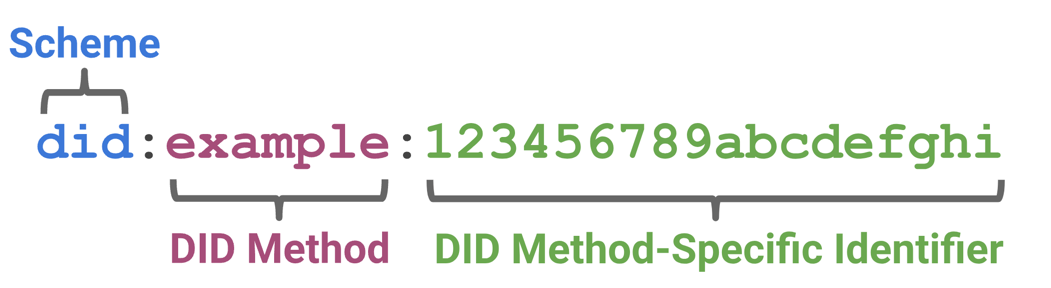
\includegraphics[width=0.7\textwidth]{figures/parts-of-a-did.png}
    \caption{Structure of a Decentralized Identifier~\cite{did}}\label{fig:did_structure}
\end{figure}

\begin{figure}
\centering
\begin{minted}[bgcolor=LightGray,breaklines]{json}
{
  "@context": [
    "https://www.w3.org/ns/did/v1",
    "https://w3id.org/security/suites/jws-2020/v1"
  ],
  "id": "did:web:gaia-x-dev.simerda.dev:gaia-x:john-doe",
  "verificationMethod": [
    {
      "id": "did:web:gaia-x-dev.simerda.dev:gaia-x:john-doe#JWK2020-RSA",
      "type": "JsonWebKey2020",
      "controller": "did:web:gaia-x-dev.simerda.dev:gaia-x:john-doe",
      "publicKeyJwk": {
        "kty": "RSA",
        "n": "1BQuEryN-A0p-TI8HOtN5xB8rwbyUre4e0fhUiPECFvd58xX_gsiMFqrsDb3ZcrnaE-0o4StXy5A0GFBouuwGX1UlZQ1V9PiPXbd05vAbv4T7xGeAuzhDbgZviiJb-SsLFAZQc6UDC5eeM1x7_KWgRCB82Nc9BGfCxLz3U6dyzrUZq8VKn9S3mkKLLuslewa00X8TCHEAVQFEktVV9F617GXEknrEZhKoZfPeuiweMj4FxuamBRQPaZlCWQduiDnVkmNu4pr7C7HJQkBxxH-D32IhxGrSg1mQtaSO-wbYgqVMoDyWFmdUGoiQmocXWKwRBC0zuxvxgninAB7wTywbQ",
        "e": "AQAB",
        "alg": "RS256",
        "x5u": "https://gaia-x-dev.simerda.dev/gaia-x/john-doe/cert.pem"
      }
    }
  ],
  "assertionMethod": [
    "did:web:gaia-x-dev.simerda.dev:gaia-x:john-doe#JWK2020-RSA"
  ]
}
\end{minted}
\caption{Example of a DID document}\label{fig:did_document}
\end{figure}

\subsection{Trust Anchors}\label{subsec:trust-anchors}

Trust Anchors are entities that underpin the claims by Participants and are endorsed by Gaia-X~\cite{gaiax_trust_framework}.
They facilitate the processing of claims made by Participants and shall do so via fair and transparent procedures and thus affirm the trust in otherwise mere self-declared statements.
Trust Anchors may underpin any aspect of the Participant's operation; however, Gaia-X will only be interested in aspects relating to criteria relevant stemming from the issued specifications.

In reality, the abstract term ``Trust Anchors'' primarily refers to the Trust Service Providers (TSPs) or Certification Authorities (CAs) from which a Participant is permitted to obtain digital certificates.
Notable exception is for the Credential \texttt(legalRegistrationNumber), where the Gaia-X Association nominated itself as a valid Trust Anchor for the purpose of validating legal person's registration numbers via the notary service.
These certificates are necessary for signing Gaia-X Credentials to ensure trust and compliance with Gaia-X standards.
The exact permissible Trust Anchors are defined in Table~\ref{tab:trust_anchors}.

\begin{figure}
    \centering
    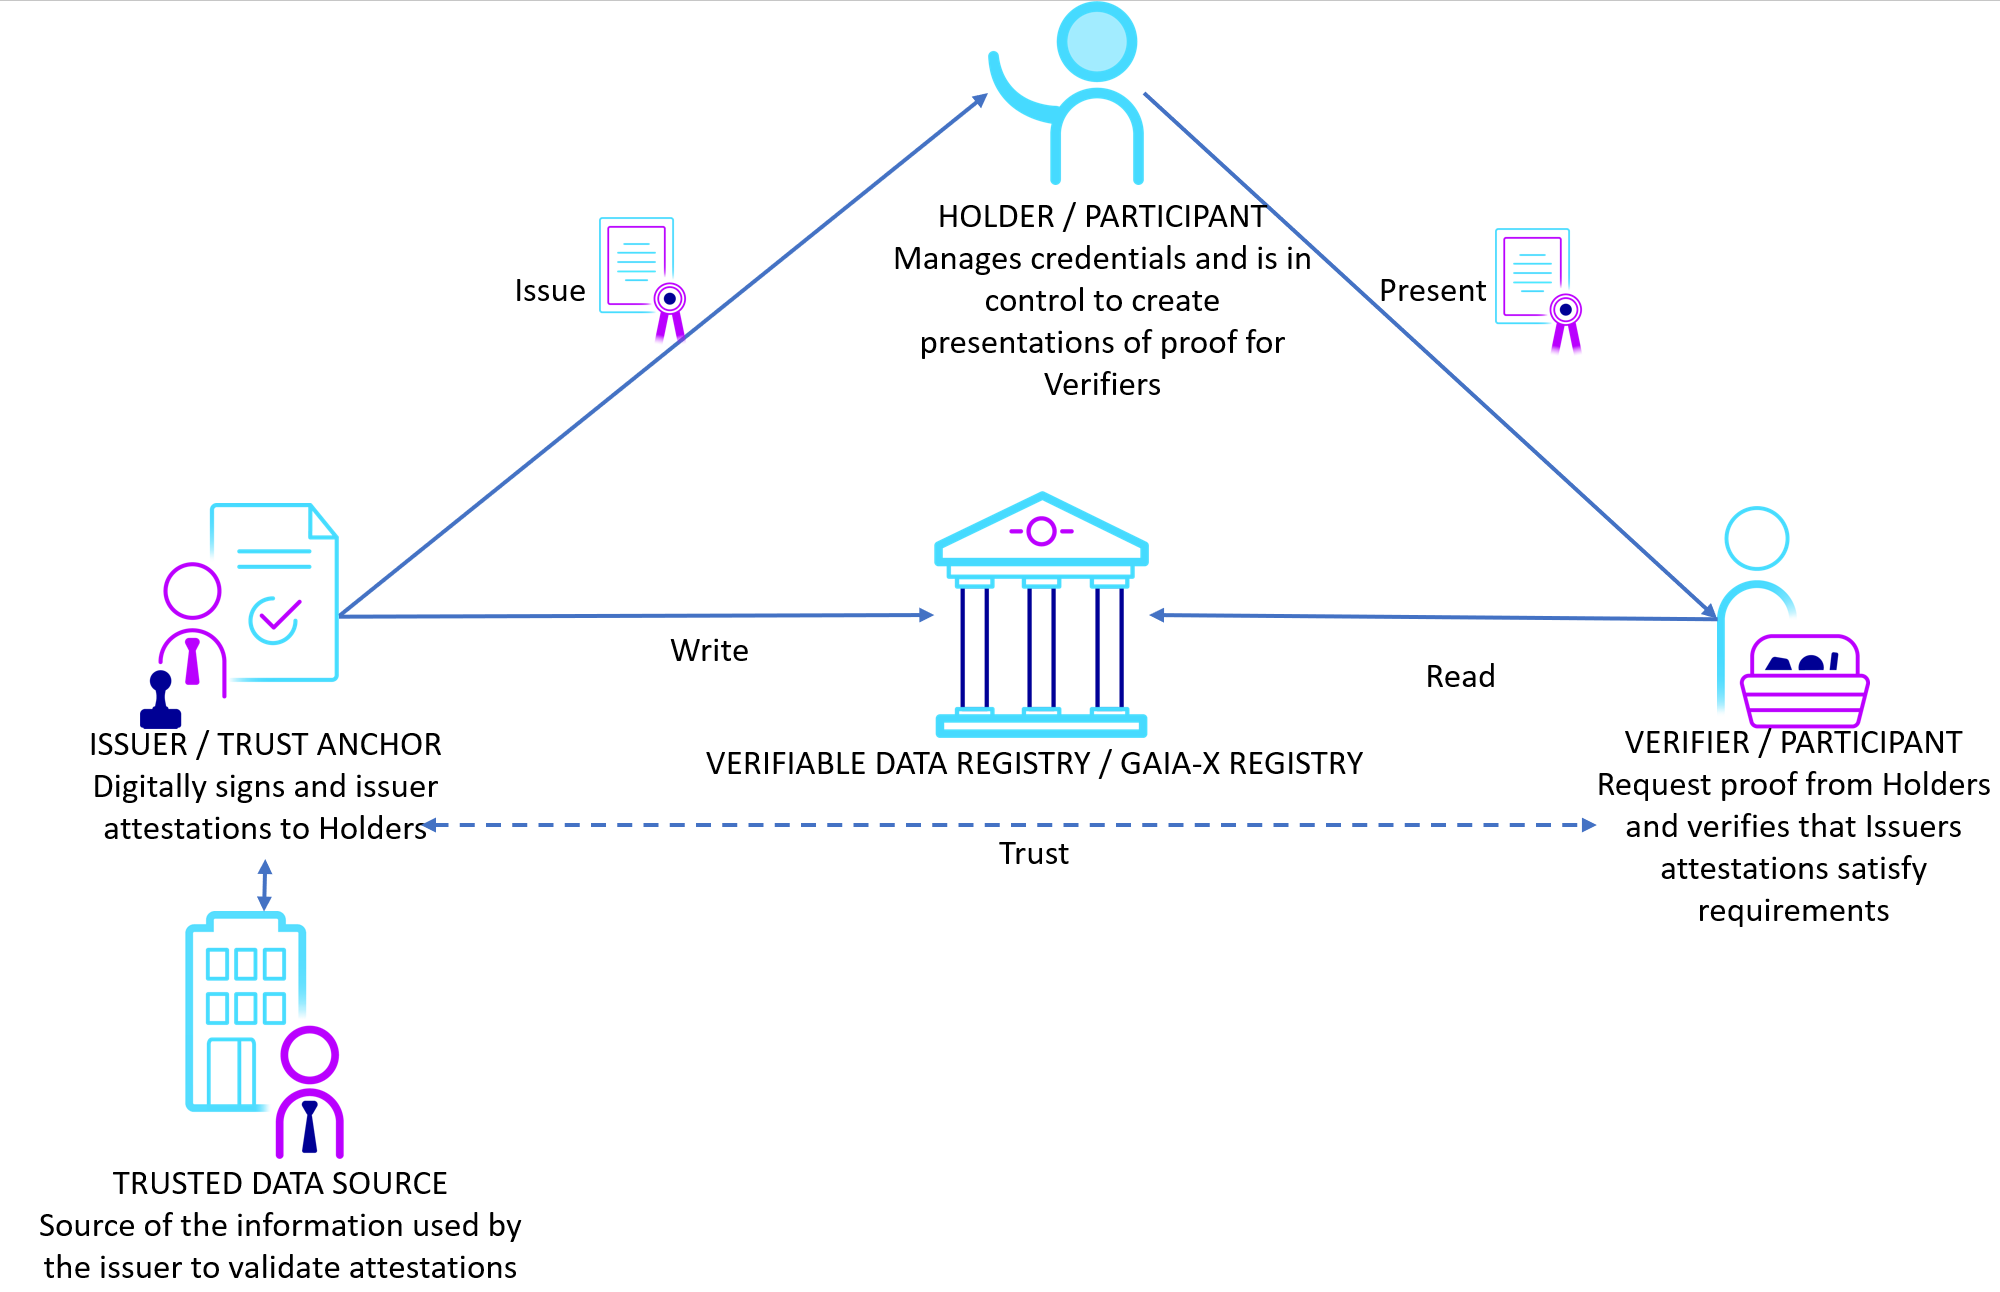
\includegraphics[width=\textwidth]{figures/vc_model.png}
    \caption{Interactions among different Participant roles in the Gaia-X Trust Framework~\cite{gaiax_trust_framework}}\label{fig:trust_framework_interactions}
\end{figure}

\begin{longtable}{ |p{4cm}|p{11cm}| }
    \hhline{--}
    \textbf{Name} & \textbf{Defined as}\\
    \hhline{--}
    State & The Trust Service Providers (TSP) must be a state validated identity issuers or EV SSL issuers.
    - For participant, if the legalAddress.country is in EEA, valid state identity issuers are eiDAS ones.
    - Gaia-X Association may also be a valid TSP for Gaia-X Association members.\\
    \hhline{--}
    eiDAS & Issuers of Qualified Certificate for Electronic Signature as defined in eIDAS Regulation (EU) No 910/2014
    (homepage: https://esignature.ec.europa.eu/efda/tl-browser/\#/screen/home)
    (machine: https://ec.europa.eu/tools/lotl/eu-lotl.xml)\\
    \hhline{--}
    EV SSL & Extended Validation (EV) Secure Sockets Layer (SSL) certificate issuers are considered to be temporarily valid Trust Service Providers.
    (homepage: https://wiki.mozilla.org/CA/Included\_Certificates)
    (machine: https://ccadb-public.secure.force.com/mozilla/IncludedCACertificateReportPEMCSV)\\
    \hhline{--}
    registrationNumberIssuer & During the pilot phase, the Gaia-X Association nominated itself as a valid Trust Anchor under https://notary.gaia-x.eu\\
    \hhline{--}
    \caption{Trust Anchors~\cite{gaiax_trust_framework}}
    \label{tab:trust_anchors}
\end{longtable}

\subsection{Policies}\label{subsec:policies}

Policies in the Gaia-X ecosystem are simply put statements, rules or assertions that specify the correct or expected behavior of an entity~\cite{gaiax_architecture_document}.
Gaia-X defines policies for all service providers and service offerings.
They specify, for example, the rules governing privacy and cybersecurity expressed indirectly in the Gaia-X specification as rules for the attributes in the Gaia-X credentials.
On top of the general policies, the Gaia-X ecosystem allows Participants to define further restrictions by using so-called policy descriptions.

The policies on the consumer side can be used to describe restrictions when searching for service or resource they want to consume; for example, the location of the service provider or a certain service level~\cite{gaiax_architecture_document}.
The provider, on the other hand, can define their own policies on the Gaia-X credentials (Service Offering, Data Resource, etc.), imposing usage restrictions on the provided service; for example, restricting the timeframe when the consumer can access provided data.
Both of these participant-defined policies are called \textit{``Policy descriptions''}.
The relation between different types of policies is visually depicted in Figure~\ref{fig:gaiax_policies}.

\begin{figure}
    \centering
    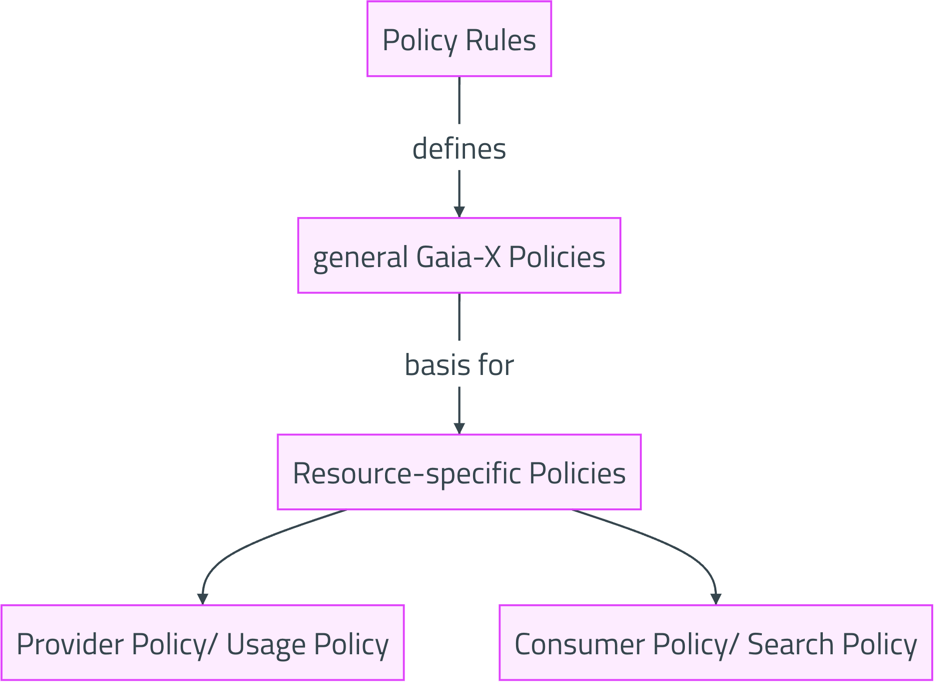
\includegraphics[width=0.7\textwidth]{figures/policies.png}
    \caption{Relation between different types of Gaia-X Policies~\cite{gaiax_architecture_document}}\label{fig:gaiax_policies}
\end{figure}

\subsubsection{Policies for Data Exchange}

A specific subset of Gaia-X policies are policies for data exchange\cite{gaiax_data_exchange_document}.
They are divided into two categories --- contract policies and runtime policies.

Contract policies server as an interoperable human and machine-readable basis for a contract between the participants.
They contain policies for access and usage control and are denoted in a ORDL DSL\footnote{Domain Specific Language is a programming language with a higher level of abstraction optimized for a specific set of problems~\cite{domain_specific_languages}.}.
ORDL is used to describe the usage control and access control policies:
\begin{itemize}
    \item \textbf{Usage control} --- regulates the obligations surrounding data processing.
    It is relevant in the context of intellectual property protection, compliance with regulations, and, more generally, digital rights management.
    For example, the following policy classes can be defined:
    \begin{itemize}
        \item Interval-restricted Data Usage
        \item Location Restricted Policy
        \item Perpetual Data Sale (Payment once)
        \item Data Rental (Payment frequently)
        \item Purpose-restricted Data Usage Policy
        \item Use Data and Delete it After (allows data usage within a specified time interval with the restriction to delete it at a specified time stamp)
        \item Attach Policy when distributing to a Third-party
        \item Distribute only if Encrypted
    \end{itemize}
    \item \textbf{Access control} --- restricts access to provided resources by defining attribute values subject must attest in order to be granted access.
\end{itemize}

Let's take a look at the main concepts of ORLD~\cite{gaiax_data_exchange_document}:
\begin{itemize}
    \item \textbf{Policy} --- Groups a set of rules (permission, prohibitions or obligations).
    It has three subclasses:
    \begin{itemize}
        \item \textbf{Set}: A generic collection of rules
        \item \textbf{Offer}: A collection of rules offered by an actor designated by the \texttt{assigner} property
        \item \textbf{Agreement}: A collection of rules agreed upon by \texttt{assignee} and \texttt{assigner} actors
    \end{itemize}
    \item \textbf{Rule} --- Defines a rule via asset (defines the target resource), action (defines the operation to be performed), constraint (defines conditions under which the rule is valid) and party (defines actors involved in the rule).
    It has three subclasses:
    \begin{itemize}
        \item \textbf{Permission}: Grants permission for the actor to perform the action
        \item \textbf{Duty}: Obliges the actor to perform the action
        \item \textbf{Prohibition}: Prohibits the actor from performing the action
    \end{itemize}
    \item \textbf{Asset} --- Specifies a resource or a collection of resources
    \item \textbf{Action} --- Specifies an operation that can be performed on an asset.
    The main two actions are \texttt{use} and \texttt{transfer}
    \item \textbf{Constraint} --- Specifies a logical expression, allowing filtering on different collections.
    Comparison operators like \texttt{lt}, \texttt{lteq}, \texttt{eq}, \texttt{gteq} and \texttt{gt} meaning ``less than'', ``less than or equal'', ``equal'', ``greater than or equal'' and ``greater than'' respectively can be used in the expression.
    Apart from comparison operators, logical operators \texttt{or}, \texttt{xone}, \texttt{and}, \texttt{andSequence} can also be used.
    \item \textbf{Party} --- Specifies an actor or a collection of actors which have a functional role in a rule.
    An actor can have the \texttt{assignee} or the \texttt{assigner} role meaning the recipient of the rule or the issuer of the rule respectively
\end{itemize}

The Figure~\ref{fig:ordl_example} showcases a JSON-LD-formatted policy obliging the \textit{``Data Consumer''} to pay 500~\char"20AC~ and defining a duty (under the \texttt{obligation} attribute) for the \textit{``Data Consumer''} to distribute the example dataset to the \textit{``Data Consumer''}.

\begin{figure}
    \centering
    \begin{minted}[bgcolor=LightGray,breaklines]{json}
{
 "@context": "https://www.w3.org/ns/odrl.jsonld",
 "@type": "Set",
 "uid": "https://data-exchange.com/policy:1",
 "permission": [
   {
     "target": "https://data-exchange.com/dataset/123",
     "assignee": "Data Consumer",
     "action": "use",
     "duty": [
       {
         "assigner": "Data Provider",
         "assignee": "Data Consumer",
         "action": [
           {
             "value": "compensate",
             "refinement": [
               {
                 "leftOperand": "payAmount",
                 "operator": "eq",
                 "rightOperand": { "@value": "500.00", "@type": "xsd:decimal" },
                 "unit": "https://dbpedia.org/resource/Euro"
               }
             ]
           }
         ]
       }
     ]
   }
 ],
 "obligation": [
   {
     "target": "https://data-exchange.com/dataset/123",
     "assigner": "Data Consumer",
     "assignee": "Data Provider",
     "action": "distribute"
   }
 ]
}
    \end{minted}
    \caption{Example of an ORDL policy obliging the \textit{``Data Provider''} to provide a dataset upon \textit{``Data Consumer's''} payment of 500~\char"20AC~~\cite{gaiax_data_exchange_document}}\label{fig:ordl_example}
\end{figure}


Outside of data exchange, runtime policies are described using a REGO DSL --- declarative language used for specifying so-called \textit{decisions}, which describe the conditions under which access is allowed or disallowed respectively.
A \textit{policy engine} is then used for executing queries over the policy, which can be used by consumer to filter desired service offering.
An example of a REGO policy modifying data retention and data policy can be seen in Figure~\ref{fig:rego_policy_example}.

\begin{figure}
    \centering
    \begin{minted}[bgcolor=LightGray,breaklines]{prolog}
default allow := false

allow if {
   shortRetention
   locatedInEEA
}

shortRetention if input.DataRetention < data.maxDataRetention

locatedInEEA if input.processingLocation.countryCode == data.EEA[_][_]
    \end{minted}
    \caption{Example of a REGO policy specifying required data retention and data location~\cite{gaiax_compliance_as_a_code}}\label{fig:rego_policy_example}
\end{figure}

The fact that policies in Gaia-X are defined in a machine-readable way allows for automated contract negotiation between provider and consumer~\cite{gaiax_data_exchange_document}.
The consumer can search for the desired service offering, initiate a contract negotiation sequence and exchange counter-offers until and agreement is reached, which is confirmed by all participants electronically signing the contract.

\subsection{Trust Framework Components}\label{subsec:trust-framework-components}

This section describes the software components which are operated by the Gaia-X Digital Clearing Houses (GXDCHs).
Gaia-X Digital Clearing House~\cite{gaiax} is a term describing a network of execution nodes, they operationalize the theoretical Gaia-X Framework by enforcing the set of rules defined in Gaia-X specifications and provide a Gaia-X compliance.
Along with \textit{Gaia-X Lab}\footnote{A team of developers working under the umbrella of the Gaia-X Association}, the services are operated by four other companies, making it a decentralized system.
The GXCHs consist of three mandatory services --- Gaia-X Compliance, Gaia-X Registry and Gaia-X Notary.

\subsubsection{Gaia-X Compliance}

The purpose of this service is to accept Gaia-X Credentials (wrapped in a Verifiable Presentation), check them against the defined schemas and verify the validity of the Credentials using syntactic, consistency and cryptographical checks~\cite{gaiax_trust_framework}.
If all the checks pass, the service returns a Gaia-X Credential with a Gaia-X signature, as a proof that the input provided has passed all the verifications, proving Participant's compliance.

\subsubsection{Gaia-X Registry}

The Registry is a backbone of the Gaia-X ecosystem governance, acting as a non-repudiable, immutable and permissionless database\cite{gaiax_trust_framework}.
The database stores the following information:
\begin{itemize}
    \item the list of the Trust Anchors – keyring.
    \item the result of the Trust Anchors validation processes.
    \item the potential revocation of Trust Anchors' identity.
    \item the vote and results of the Gaia-X Association roll call vote, similar to the rules of the plenary of the European Parliament.
    \item the shapes and schemas for the Gaia-X VCs.
    \item the URLs of Gaia-X Catalogue’s credentials.
    \item the text of the Terms and Conditions for Gaia-X Conformity.
\end{itemize}

\subsubsection{Gaia-X Notary}

At the moment, the Notary service serves the singular purpose of validating the Participant's legal registration number~\cite{gaiax_trust_framework}.
It checks that the Gaia-X credential contains at least one of the permissible legal entity identification number stated in the Gaia-X specifications and validates it using external services.
Upon successful validation, it issues a Gaia-X Credential attesting to these claims.

In the future, the notary shall also perform notarization of Data Product Usage Contracts. %TODO: cite data exchange specification

\section{Implementation}\label{sec:implementation}

\textcolor{red}{This will be probably a shorter section about my concrete implementation of the data exchange module in the context of Carecentive.}

\section{Evaluation}\label{sec:evaluation}

In order to evaluate the actual state of the Gaia-X ecosystem, the following tests will be performed with using our implementation of the Carecentive exchange module.

\begin{enumerate}
    \item Obtaining Gaia-X compliance
    \item Creating Gaia-X credentials for data products
    \item Performing data exchange with questionnaire data
    \item Performing data exchange with withings data
\end{enumerate}

The results of these tests are presented in the following chapter.
